% Seminar 6: VAR models and Granger causality
% Time Series Analysis -- Bachelor's programmes Economic Informatics and Economic Cybernetics, Bucharest University of Economic Studies
% GENERATED by latex/build_seminar6.py -- edit the generator, not this file.
% Student version by default; the instructor version is the *_solutions.tex wrapper.
\makeatletter\@ifundefined{ifsolutions}{\expandafter\newif\csname ifsolutions\endcsname}{}\makeatother

\newcommand{\coursename}{Time Series Analysis}
% Preambul comun TSA -- Serii de timp / Time Series Analysis (Beamer, 16:9)
% Același design ca MFM și SFM (preluat din SFM, 5 octombrie 2026). Înainte de % Preambul comun TSA -- Serii de timp / Time Series Analysis (Beamer, 16:9)
% Același design ca MFM și SFM (preluat din SFM, 5 octombrie 2026). Înainte de % Preambul comun TSA -- Serii de timp / Time Series Analysis (Beamer, 16:9)
% Același design ca MFM și SFM (preluat din SFM, 5 octombrie 2026). Înainte de \input{../../latex/preamble} se definește
%   \newcommand{\coursename}{Time Series Analysis}      (EN)
%   \newcommand{\coursename}{Serii de timp}       (RO)  și  \def\tsalang{ro}
% Fișierele .tex se află în EN/Courses, EN/Seminars, RO/Cursuri, RO/Seminarii (două niveluri sub rădăcină).
% Deck-urile sînt generate de latex/build_chapterN.py / build_seminarN.py (vezi latex/tsa_build.py).

\documentclass[9pt, aspectratio=169, t]{beamer}
\providecommand{\coursename}{Time Series Analysis}

% Ensure content fits on slides
\setbeamersize{text margin left=8mm, text margin right=8mm}
% Smaller institute font (title page)
\setbeamerfont{institute}{size=\footnotesize}

%=============================================================================
% THEME AND STYLE CONFIGURATION
%=============================================================================
\usetheme{default}
% Using default theme for clean header/footer control

% Color Palette (matching Redispatch PDF)
\definecolor{MainBlue}{RGB}{26, 58, 110}
\definecolor{AccentBlue}{RGB}{26, 58, 110}
\definecolor{IDAred}{RGB}{205, 0, 0}
\definecolor{DarkGray}{RGB}{51, 51, 51}
\definecolor{MediumGray}{RGB}{128, 128, 128}
\definecolor{LightGray}{RGB}{248, 248, 248}
\definecolor{VeryLightGray}{RGB}{235, 235, 235}
\definecolor{KeynoteGray}{RGB}{218, 218, 218}
\definecolor{SectionGray}{RGB}{120, 120, 120}
\definecolor{FooterGray}{RGB}{100, 100, 100}
\definecolor{Crimson}{RGB}{220, 53, 69}
\definecolor{Forest}{RGB}{46, 125, 50}
\definecolor{Amber}{RGB}{181, 133, 63}
\definecolor{Orange}{RGB}{230, 126, 34}
\definecolor{Purple}{RGB}{142, 68, 173}

% Gradient background (exact Keynote 315° gradient: white to RGB 218,218,218)
\setbeamertemplate{background}{%
    \begin{tikzpicture}[remember picture, overlay]
        \shade[shading=axis, shading angle=315,
        top color=white, bottom color=KeynoteGray]
        (current page.south west) rectangle (current page.north east);
    \end{tikzpicture}%
}
% Fallback solid color for compatibility
\setbeamercolor{background canvas}{bg=}

\setbeamercolor{palette primary}{bg=MainBlue, fg=white}
\setbeamercolor{palette secondary}{bg=MainBlue!85, fg=white}
\setbeamercolor{palette tertiary}{bg=MainBlue!70, fg=white}
\setbeamercolor{structure}{fg=MainBlue}
\setbeamercolor{title}{fg=IDAred}
\setbeamercolor{frametitle}{fg=IDAred, bg=}
\setbeamercolor{block title}{bg=MainBlue, fg=white}
\setbeamercolor{block body}{bg=VeryLightGray, fg=DarkGray}
\setbeamercolor{block title alerted}{bg=Crimson, fg=white}
\setbeamercolor{block body alerted}{bg=Crimson!8, fg=DarkGray}
\setbeamercolor{block title example}{bg=Forest, fg=white}
\setbeamercolor{block body example}{bg=Forest!8, fg=DarkGray}
\setbeamercolor{item}{fg=MainBlue}

% Footer colors (override Madrid theme blue)
\setbeamercolor{author in head/foot}{fg=FooterGray, bg=}
\setbeamercolor{title in head/foot}{fg=FooterGray, bg=}
\setbeamercolor{date in head/foot}{fg=FooterGray, bg=}
\setbeamercolor{section in head/foot}{fg=FooterGray, bg=}
\setbeamercolor{subsection in head/foot}{fg=FooterGray, bg=}

% Bullet styles (apply everywhere including blocks)
\setbeamertemplate{itemize item}{\color{MainBlue}$\boxdot$}
\setbeamertemplate{itemize subitem}{\color{MainBlue}$\blacktriangleright$}
\setbeamertemplate{itemize subsubitem}{\color{MainBlue}\tiny$\bullet$}
\setbeamertemplate{itemize/enumerate body begin}{\normalsize}
\setbeamertemplate{itemize/enumerate subbody begin}{\normalsize}

% Item spacing - compact style
\setlength{\leftmargini}{10pt}       % Level 1: minimal indent
\setlength{\leftmarginii}{10pt}      % Level 2: minimal additional indent
% Compact list spacing (zero extra space before/after lists in blocks)
\makeatletter
\def\@listi{\leftmargin\leftmargini \topsep 0pt \parsep 0pt \itemsep 0pt}
\def\@listii{\leftmargin\leftmarginii \topsep 0pt \parsep 0pt \itemsep 0pt}
\makeatother

\setbeamertemplate{navigation symbols}{}

%=============================================================================
% CUSTOM HEADLINE
%=============================================================================
\setbeamertemplate{headline}{%
    \vskip10pt%
    \hbox to \paperwidth{%
        \hskip0.5cm%
        {\small\color{FooterGray}\renewcommand{\hyperlink}[2]{##2}\insertsectionhead}%
        \hfill%
        \textcolor{FooterGray}{\small\insertframenumber}%
        \hskip0.5cm%
    }%
    \vskip4pt%
    {\color{FooterGray}\hrule height 0.4pt}%
}

%=============================================================================
% CUSTOM FOOTER
%=============================================================================
\usepackage{fontawesome5}

\setbeamertemplate{footline}{%
    {\color{FooterGray}\hrule height 0.4pt}%
    \vskip4pt%
    \hbox to \paperwidth{%
        \hskip0.5cm%
        \textcolor{FooterGray}{\small\coursename}%
        \hfill%
        \raisebox{-0.1em}{%
            \begin{tikzpicture}[x=0.08em, y=0.08em, line width=0.4pt]
                \draw[FooterGray] (0,3) -- (1,4) -- (2,3.5) -- (3,5) -- (4,4) -- (5,6) -- (6,5.5) -- (7,4) -- (8,5) -- (9,7) -- (10,6) -- (11,5) -- (12,6.5) -- (13,8) -- (14,7) -- (15,6) -- (16,7.5) -- (17,9) -- (18,8) -- (19,7) -- (20,8.5) -- (21,10) -- (22,9) -- (23,8) -- (24,9.5);
            \end{tikzpicture}%
        }%
        \hskip0.5cm%
    }%
    \vskip6pt%
}

%=============================================================================
% PACKAGES
%=============================================================================
\usepackage[utf8]{inputenc}
\DeclareUnicodeCharacter{03B1}{\ensuremath{\alpha}}
\usepackage[T1]{fontenc}
\usepackage{amsmath, amssymb, amsthm}
\usepackage{mathtools}
\usepackage{bm}
\usepackage{tikz}
\usetikzlibrary{arrows.meta, positioning, shapes, calc, decorations.pathreplacing, shadings}
\usepackage{booktabs}
\usepackage{multirow}
\usepackage{array}
\usepackage{graphicx}
\usepackage{animate}
\usepackage{hyperref}
\usepackage{colortbl}
\usepackage{listings}
\lstset{language=Python, basicstyle=\ttfamily\scriptsize, keywordstyle=\color{MainBlue}\bfseries,
  commentstyle=\color{Forest}, stringstyle=\color{Crimson}, breaklines=true,
  frame=none, backgroundcolor=\color{VeryLightGray}, xleftmargin=2mm}
\hypersetup{colorlinks=true, linkcolor=MainBlue, urlcolor=MainBlue}
\graphicspath{{../../logos/}{../../charts/}{../../photos/}}
\usepackage{xcolor}
\hfuzz=2pt  % Suppress tiny overfull warnings (<2pt)
\vfuzz=2pt  % Suppress tiny vertical overfull warnings (<2pt)
% \mathrm in the sans-serif family of the slides (beamer resets \mathrm to the serif family at \begin{document};
% this hook runs after beamer's, so WN, Var, RMSE, ... in formulas match the surrounding text)
% Bold vectors and matrices in the same sans-serif family: \mathbf{A} in sans bold (beamer's own \mathbf came out in
% medium weight), and the bold upright Greek capitals of \boldsymbol / \bm (\bSigma, \bPhi, \boldsymbol{\Theta}) in
% cmss bold: bm.sty fixes its "boldoperators" font when it is loaded (serif cmbx), before beamer switches the
% operators to cmss, so it is reset here.
\AtBeginDocument{%
  \SetMathAlphabet{\mathrm}{normal}{\encodingdefault}{\sfdefault}{\mddefault}{n}%
  \SetMathAlphabet{\mathrm}{bold}{\encodingdefault}{\sfdefault}{bx}{n}%
  \SetMathAlphabet{\mathbf}{normal}{\encodingdefault}{\sfdefault}{bx}{n}%
  \SetMathAlphabet{\mathbf}{bold}{\encodingdefault}{\sfdefault}{bx}{n}%
  \SetSymbolFont{boldoperators}{normal}{OT1}{cmss}{bx}{n}%
  \SetSymbolFont{boldoperators}{bold}{OT1}{cmss}{bx}{n}}

%=============================================================================
% QUANTLET COMMANDS
%   \quantlet{<displayed name>}{<url>}       (generic, compatible with the older TSA decks)
%   \tsaquantlet{Ch_05}{TSA_ch5_garch}       -> https://github.com/danpele/Time-Series-Analysis/tree/main/Quantlets/Ch_05/TSA_ch5_garch
%   \qlurl{<folder>} is defined per chapter by the generator (Quantlets/Ch_NN/<folder>)
%=============================================================================
\newcommand{\tsarepo}{https://github.com/danpele/Time-Series-Analysis}
\newcommand{\tsaqlbase}{https://github.com/danpele/Time-Series-Analysis/tree/main/Quantlets}
\newcommand{\quantlet}[2]{%
    \hfill\href{#2}{%
        \raisebox{-0.15em}{
\includegraphics[height=0.7em]{ql_logo.png}}%
        \textcolor{MainBlue}{\tiny\ #1}%
    }%
}
\newcommand{\tsaquantlet}[2]{\quantlet{\detokenize{#2}}{\tsaqlbase/#1/#2}}

%=============================================================================
% NOTEBOOKS (Google Colab)
%   \colaburl{notebooks/EN/chapter5_seminar_notebook.ipynb} -> the Colab link of a file in the TSA repo
%   \nb: the chapter notebook (each seminar deck redefines it with \renewcommand)
%=============================================================================
\newcommand{\colaburl}[1]{https://colab.research.google.com/github/danpele/Time-Series-Analysis/blob/main/#1}
\newcommand{\nb}{https://colab.research.google.com/github/danpele/Time-Series-Analysis/tree/main/notebooks/EN}
\newcommand{\nbname}{notebooks/EN}

%=============================================================================
% SLIDE HELPERS (used by the generators; the same as in MFM)
%=============================================================================
% local font size for list bodies (the preamble forces \normalsize)
\newcommand{\itemsize}[1]{\setbeamertemplate{itemize/enumerate body begin}{#1}\setbeamertemplate{itemize/enumerate subbody begin}{#1}}
\newcommand{\intitle}[1]{{\hypersetup{urlcolor=white}#1}}   % white links inside coloured title bars
\newcommand{\imgcap}[1]{{\scriptsize #1}\\[0.5mm]}          % caption under a photo
\newcommand{\imgcredit}[2]{{\tiny\color{FooterGray}\href{#1}{#2}}}   % image credit: source URL, author/licence
\newcommand{\aiprompt}[1]{{\ttfamily\color{MainBlue}#1}}     % a prompt to an AI assistant

%=============================================================================
% SEMINARS: student version by default; the instructor wrapper *_solutions.tex sets \solutionstrue
%=============================================================================
\makeatletter\@ifundefined{ifsolutions}{\expandafter\newif\csname ifsolutions\endcsname}{}\makeatother
\newcommand{\solonly}[1]{\ifsolutions #1\fi}
\newcommand{\propsub}{\ifsolutions\else\framesubtitle{\ifdefined\tsalang Rezolvarea se discută la seminar\else Solution discussed in class\fi}\fi}

%=============================================================================
% APPENDIX AND CHAPTER LINKS (latex/appendix_links.py writes the calls; it also re-declares these
% macros before \begin{document}, so the decks compile with or without this preamble block)
%=============================================================================
\providecommand{\tsaapplink}[3]{\hypertarget{#2}{}\hyperlink{#1}{\beamergotobutton{#3}}}
\providecommand{\tsaappback}[2]{\begin{tikzpicture}[remember picture,overlay]\node[anchor=south east] at ([xshift=-3mm,yshift=7mm]current page.south east){\hyperlink{#1}{\beamerreturnbutton{#2}}};\end{tikzpicture}}
\providecommand{\tsachlink}[2]{\href{#1}{#2}}
\providecommand{\tsachlinkt}[2]{\href{#1}{\usebeamercolor[fg]{frametitle}#2}}

%=============================================================================
% QUANTINAR COMMAND: link către un curs Quantinar (subiecte avansate)
%=============================================================================
\newcommand{\quantinar}[2]{%
    \href{#2}{%
        \raisebox{-0.15em}{
\includegraphics[height=0.8em]{qr_logo.png}}%
        \textcolor{MainBlue}{\scriptsize\ #1}%
    }%
}

%=============================================================================
% CUSTOM TITLE PAGE
%=============================================================================
\defbeamertemplate*{title page}{hybrid}[1][]
{
    \vspace{0.2cm}
    % Logos row - top header (with clickable links)
    \begin{center}
        \href{https://www.ase.ro}{
\includegraphics[height=1.0cm]{ase_logo.png}}\hspace{0.3cm}%
        \href{https://theida.net}{
\includegraphics[height=1.0cm]{ida_logo.png}}\hspace{0.3cm}%
        \href{https://blockchain-research-center.com}{
\includegraphics[height=1.0cm]{brc_logo.png}}\hspace{0.3cm}%
        \href{https://www.ai4efin.ase.ro}{
\includegraphics[height=1.0cm]{ai4efin_logo.png}}\hspace{0.3cm}%
        \href{https://ipe.ro/new}{
\includegraphics[height=1.0cm]{acad_logo.png}}\hspace{0.3cm}%
        \href{https://www.digital-finance-msca.com}{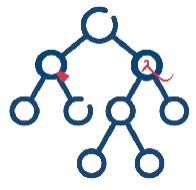
\includegraphics[height=1.0cm]{msca_logo.png}}%
    \end{center}

    \vspace{0.6cm}

    % Main title with Q logos on sides (with clickable links)
    \begin{center}
        \begin{minipage}{0.1\textwidth}
            \centering
            \href{https://quantlet.com}{
\includegraphics[height=1.1cm]{ql_logo.png}}
        \end{minipage}%
        \begin{minipage}{0.78\textwidth}
            \centering
            {\LARGE\bfseries\usebeamercolor[fg]{title}\inserttitle}

            \vspace{0.3cm}

            {\usebeamerfont{subtitle}\usebeamercolor[fg]{title}\insertsubtitle}
        \end{minipage}%
        \begin{minipage}{0.1\textwidth}
            \centering
            \href{https://quantinar.com}{
\includegraphics[height=1.1cm]{qr_logo.png}}
        \end{minipage}
    \end{center}

    \vspace{0.6cm}

    % Authors (left aligned)
    \hspace{0.5cm}{\usebeamerfont{author}\insertauthor}

    \vspace{0.3cm}

    % Institute/Affiliations (left aligned)
    \hspace{0.5cm}\begin{minipage}[t]{0.9\textwidth}
        \raggedright\small\insertinstitute
    \end{minipage}
}

%=============================================================================
% THEOREM ENVIRONMENTS
%=============================================================================
\theoremstyle{definition}
\setbeamertemplate{theorems}[numbered]
\ifdefined\tsalang
\newtheorem{defn}{Definiție}
\newtheorem{thm}{Teoremă}
\newtheorem{prop}{Propoziție}
\newtheorem{rmk}{Observație}
\else
\newtheorem{defn}{Definition}
\newtheorem{thm}{Theorem}
\newtheorem{prop}{Proposition}
\newtheorem{rmk}{Remark}
\fi

%=============================================================================
% CENTRED MINIPAGE (no extra vertical space)
%=============================================================================
\newenvironment{cminipage}[1]{%
    \par\noindent\hfill\begin{minipage}{#1}\ignorespaces
}{%
    \end{minipage}\hfill\null\par
}

%=============================================================================
% CUSTOM COMMANDS
%=============================================================================
\newcommand{\E}{\mathbb{E}}
\newcommand{\Var}{\text{Var}}
\newcommand{\Cov}{\text{Cov}}
\newcommand{\Corr}{\text{Corr}}
\newcommand{\R}{\mathbb{R}}
\newcommand{\N}{\mathbb{N}}
\newcommand{\Z}{\mathbb{Z}}
\newcommand{\B}{\mathbf{B}}
\newcommand{\imark}{\textcolor{MainBlue}{\textbullet}}
\newcommand{\RMSE}{\text{RMSE}}
\newcommand{\MAE}{\text{MAE}}
\newcommand{\MAPE}{\text{MAPE}}

% Boldface vector/matrix commands (VAR, VECM, state space; also used by the older TSA decks)
\newcommand{\bY}{\mathbf{Y}}
\newcommand{\bX}{\mathbf{X}}
\newcommand{\bA}{\mathbf{A}}
\newcommand{\bB}{\mathbf{B}}
\newcommand{\bepsilon}{\boldsymbol{\varepsilon}}
\newcommand{\bSigma}{\boldsymbol{\Sigma}}
\newcommand{\bPhi}{\boldsymbol{\Phi}}
\newcommand{\bGamma}{\boldsymbol{\Gamma}}
\newcommand{\bPi}{\boldsymbol{\Pi}}
\newcommand{\bc}{\mathbf{c}}
\newcommand{\balpha}{\boldsymbol{\alpha}}
\newcommand{\bbeta}{\boldsymbol{\beta}}
\newcommand{\bvarepsilon}{\boldsymbol{\varepsilon}}

% Legacy seminar marks (older TSA seminar decks)
\newcommand{\correct}{\textcolor{Forest}{\checkmark}}
\newcommand{\incorrect}{\textcolor{Crimson}{\texttimes}}
 se definește
%   \newcommand{\coursename}{Time Series Analysis}      (EN)
%   \newcommand{\coursename}{Serii de timp}       (RO)  și  \def\tsalang{ro}
% Fișierele .tex se află în EN/Courses, EN/Seminars, RO/Cursuri, RO/Seminarii (două niveluri sub rădăcină).
% Deck-urile sînt generate de latex/build_chapterN.py / build_seminarN.py (vezi latex/tsa_build.py).

\documentclass[9pt, aspectratio=169, t]{beamer}
\providecommand{\coursename}{Time Series Analysis}

% Ensure content fits on slides
\setbeamersize{text margin left=8mm, text margin right=8mm}
% Smaller institute font (title page)
\setbeamerfont{institute}{size=\footnotesize}

%=============================================================================
% THEME AND STYLE CONFIGURATION
%=============================================================================
\usetheme{default}
% Using default theme for clean header/footer control

% Color Palette (matching Redispatch PDF)
\definecolor{MainBlue}{RGB}{26, 58, 110}
\definecolor{AccentBlue}{RGB}{26, 58, 110}
\definecolor{IDAred}{RGB}{205, 0, 0}
\definecolor{DarkGray}{RGB}{51, 51, 51}
\definecolor{MediumGray}{RGB}{128, 128, 128}
\definecolor{LightGray}{RGB}{248, 248, 248}
\definecolor{VeryLightGray}{RGB}{235, 235, 235}
\definecolor{KeynoteGray}{RGB}{218, 218, 218}
\definecolor{SectionGray}{RGB}{120, 120, 120}
\definecolor{FooterGray}{RGB}{100, 100, 100}
\definecolor{Crimson}{RGB}{220, 53, 69}
\definecolor{Forest}{RGB}{46, 125, 50}
\definecolor{Amber}{RGB}{181, 133, 63}
\definecolor{Orange}{RGB}{230, 126, 34}
\definecolor{Purple}{RGB}{142, 68, 173}

% Gradient background (exact Keynote 315° gradient: white to RGB 218,218,218)
\setbeamertemplate{background}{%
    \begin{tikzpicture}[remember picture, overlay]
        \shade[shading=axis, shading angle=315,
        top color=white, bottom color=KeynoteGray]
        (current page.south west) rectangle (current page.north east);
    \end{tikzpicture}%
}
% Fallback solid color for compatibility
\setbeamercolor{background canvas}{bg=}

\setbeamercolor{palette primary}{bg=MainBlue, fg=white}
\setbeamercolor{palette secondary}{bg=MainBlue!85, fg=white}
\setbeamercolor{palette tertiary}{bg=MainBlue!70, fg=white}
\setbeamercolor{structure}{fg=MainBlue}
\setbeamercolor{title}{fg=IDAred}
\setbeamercolor{frametitle}{fg=IDAred, bg=}
\setbeamercolor{block title}{bg=MainBlue, fg=white}
\setbeamercolor{block body}{bg=VeryLightGray, fg=DarkGray}
\setbeamercolor{block title alerted}{bg=Crimson, fg=white}
\setbeamercolor{block body alerted}{bg=Crimson!8, fg=DarkGray}
\setbeamercolor{block title example}{bg=Forest, fg=white}
\setbeamercolor{block body example}{bg=Forest!8, fg=DarkGray}
\setbeamercolor{item}{fg=MainBlue}

% Footer colors (override Madrid theme blue)
\setbeamercolor{author in head/foot}{fg=FooterGray, bg=}
\setbeamercolor{title in head/foot}{fg=FooterGray, bg=}
\setbeamercolor{date in head/foot}{fg=FooterGray, bg=}
\setbeamercolor{section in head/foot}{fg=FooterGray, bg=}
\setbeamercolor{subsection in head/foot}{fg=FooterGray, bg=}

% Bullet styles (apply everywhere including blocks)
\setbeamertemplate{itemize item}{\color{MainBlue}$\boxdot$}
\setbeamertemplate{itemize subitem}{\color{MainBlue}$\blacktriangleright$}
\setbeamertemplate{itemize subsubitem}{\color{MainBlue}\tiny$\bullet$}
\setbeamertemplate{itemize/enumerate body begin}{\normalsize}
\setbeamertemplate{itemize/enumerate subbody begin}{\normalsize}

% Item spacing - compact style
\setlength{\leftmargini}{10pt}       % Level 1: minimal indent
\setlength{\leftmarginii}{10pt}      % Level 2: minimal additional indent
% Compact list spacing (zero extra space before/after lists in blocks)
\makeatletter
\def\@listi{\leftmargin\leftmargini \topsep 0pt \parsep 0pt \itemsep 0pt}
\def\@listii{\leftmargin\leftmarginii \topsep 0pt \parsep 0pt \itemsep 0pt}
\makeatother

\setbeamertemplate{navigation symbols}{}

%=============================================================================
% CUSTOM HEADLINE
%=============================================================================
\setbeamertemplate{headline}{%
    \vskip10pt%
    \hbox to \paperwidth{%
        \hskip0.5cm%
        {\small\color{FooterGray}\renewcommand{\hyperlink}[2]{##2}\insertsectionhead}%
        \hfill%
        \textcolor{FooterGray}{\small\insertframenumber}%
        \hskip0.5cm%
    }%
    \vskip4pt%
    {\color{FooterGray}\hrule height 0.4pt}%
}

%=============================================================================
% CUSTOM FOOTER
%=============================================================================
\usepackage{fontawesome5}

\setbeamertemplate{footline}{%
    {\color{FooterGray}\hrule height 0.4pt}%
    \vskip4pt%
    \hbox to \paperwidth{%
        \hskip0.5cm%
        \textcolor{FooterGray}{\small\coursename}%
        \hfill%
        \raisebox{-0.1em}{%
            \begin{tikzpicture}[x=0.08em, y=0.08em, line width=0.4pt]
                \draw[FooterGray] (0,3) -- (1,4) -- (2,3.5) -- (3,5) -- (4,4) -- (5,6) -- (6,5.5) -- (7,4) -- (8,5) -- (9,7) -- (10,6) -- (11,5) -- (12,6.5) -- (13,8) -- (14,7) -- (15,6) -- (16,7.5) -- (17,9) -- (18,8) -- (19,7) -- (20,8.5) -- (21,10) -- (22,9) -- (23,8) -- (24,9.5);
            \end{tikzpicture}%
        }%
        \hskip0.5cm%
    }%
    \vskip6pt%
}

%=============================================================================
% PACKAGES
%=============================================================================
\usepackage[utf8]{inputenc}
\DeclareUnicodeCharacter{03B1}{\ensuremath{\alpha}}
\usepackage[T1]{fontenc}
\usepackage{amsmath, amssymb, amsthm}
\usepackage{mathtools}
\usepackage{bm}
\usepackage{tikz}
\usetikzlibrary{arrows.meta, positioning, shapes, calc, decorations.pathreplacing, shadings}
\usepackage{booktabs}
\usepackage{multirow}
\usepackage{array}
\usepackage{graphicx}
\usepackage{animate}
\usepackage{hyperref}
\usepackage{colortbl}
\usepackage{listings}
\lstset{language=Python, basicstyle=\ttfamily\scriptsize, keywordstyle=\color{MainBlue}\bfseries,
  commentstyle=\color{Forest}, stringstyle=\color{Crimson}, breaklines=true,
  frame=none, backgroundcolor=\color{VeryLightGray}, xleftmargin=2mm}
\hypersetup{colorlinks=true, linkcolor=MainBlue, urlcolor=MainBlue}
\graphicspath{{../../logos/}{../../charts/}{../../photos/}}
\usepackage{xcolor}
\hfuzz=2pt  % Suppress tiny overfull warnings (<2pt)
\vfuzz=2pt  % Suppress tiny vertical overfull warnings (<2pt)
% \mathrm in the sans-serif family of the slides (beamer resets \mathrm to the serif family at \begin{document};
% this hook runs after beamer's, so WN, Var, RMSE, ... in formulas match the surrounding text)
% Bold vectors and matrices in the same sans-serif family: \mathbf{A} in sans bold (beamer's own \mathbf came out in
% medium weight), and the bold upright Greek capitals of \boldsymbol / \bm (\bSigma, \bPhi, \boldsymbol{\Theta}) in
% cmss bold: bm.sty fixes its "boldoperators" font when it is loaded (serif cmbx), before beamer switches the
% operators to cmss, so it is reset here.
\AtBeginDocument{%
  \SetMathAlphabet{\mathrm}{normal}{\encodingdefault}{\sfdefault}{\mddefault}{n}%
  \SetMathAlphabet{\mathrm}{bold}{\encodingdefault}{\sfdefault}{bx}{n}%
  \SetMathAlphabet{\mathbf}{normal}{\encodingdefault}{\sfdefault}{bx}{n}%
  \SetMathAlphabet{\mathbf}{bold}{\encodingdefault}{\sfdefault}{bx}{n}%
  \SetSymbolFont{boldoperators}{normal}{OT1}{cmss}{bx}{n}%
  \SetSymbolFont{boldoperators}{bold}{OT1}{cmss}{bx}{n}}

%=============================================================================
% QUANTLET COMMANDS
%   \quantlet{<displayed name>}{<url>}       (generic, compatible with the older TSA decks)
%   \tsaquantlet{Ch_05}{TSA_ch5_garch}       -> https://github.com/danpele/Time-Series-Analysis/tree/main/Quantlets/Ch_05/TSA_ch5_garch
%   \qlurl{<folder>} is defined per chapter by the generator (Quantlets/Ch_NN/<folder>)
%=============================================================================
\newcommand{\tsarepo}{https://github.com/danpele/Time-Series-Analysis}
\newcommand{\tsaqlbase}{https://github.com/danpele/Time-Series-Analysis/tree/main/Quantlets}
\newcommand{\quantlet}[2]{%
    \hfill\href{#2}{%
        \raisebox{-0.15em}{
\includegraphics[height=0.7em]{ql_logo.png}}%
        \textcolor{MainBlue}{\tiny\ #1}%
    }%
}
\newcommand{\tsaquantlet}[2]{\quantlet{\detokenize{#2}}{\tsaqlbase/#1/#2}}

%=============================================================================
% NOTEBOOKS (Google Colab)
%   \colaburl{notebooks/EN/chapter5_seminar_notebook.ipynb} -> the Colab link of a file in the TSA repo
%   \nb: the chapter notebook (each seminar deck redefines it with \renewcommand)
%=============================================================================
\newcommand{\colaburl}[1]{https://colab.research.google.com/github/danpele/Time-Series-Analysis/blob/main/#1}
\newcommand{\nb}{https://colab.research.google.com/github/danpele/Time-Series-Analysis/tree/main/notebooks/EN}
\newcommand{\nbname}{notebooks/EN}

%=============================================================================
% SLIDE HELPERS (used by the generators; the same as in MFM)
%=============================================================================
% local font size for list bodies (the preamble forces \normalsize)
\newcommand{\itemsize}[1]{\setbeamertemplate{itemize/enumerate body begin}{#1}\setbeamertemplate{itemize/enumerate subbody begin}{#1}}
\newcommand{\intitle}[1]{{\hypersetup{urlcolor=white}#1}}   % white links inside coloured title bars
\newcommand{\imgcap}[1]{{\scriptsize #1}\\[0.5mm]}          % caption under a photo
\newcommand{\imgcredit}[2]{{\tiny\color{FooterGray}\href{#1}{#2}}}   % image credit: source URL, author/licence
\newcommand{\aiprompt}[1]{{\ttfamily\color{MainBlue}#1}}     % a prompt to an AI assistant

%=============================================================================
% SEMINARS: student version by default; the instructor wrapper *_solutions.tex sets \solutionstrue
%=============================================================================
\makeatletter\@ifundefined{ifsolutions}{\expandafter\newif\csname ifsolutions\endcsname}{}\makeatother
\newcommand{\solonly}[1]{\ifsolutions #1\fi}
\newcommand{\propsub}{\ifsolutions\else\framesubtitle{\ifdefined\tsalang Rezolvarea se discută la seminar\else Solution discussed in class\fi}\fi}

%=============================================================================
% APPENDIX AND CHAPTER LINKS (latex/appendix_links.py writes the calls; it also re-declares these
% macros before \begin{document}, so the decks compile with or without this preamble block)
%=============================================================================
\providecommand{\tsaapplink}[3]{\hypertarget{#2}{}\hyperlink{#1}{\beamergotobutton{#3}}}
\providecommand{\tsaappback}[2]{\begin{tikzpicture}[remember picture,overlay]\node[anchor=south east] at ([xshift=-3mm,yshift=7mm]current page.south east){\hyperlink{#1}{\beamerreturnbutton{#2}}};\end{tikzpicture}}
\providecommand{\tsachlink}[2]{\href{#1}{#2}}
\providecommand{\tsachlinkt}[2]{\href{#1}{\usebeamercolor[fg]{frametitle}#2}}

%=============================================================================
% QUANTINAR COMMAND: link către un curs Quantinar (subiecte avansate)
%=============================================================================
\newcommand{\quantinar}[2]{%
    \href{#2}{%
        \raisebox{-0.15em}{
\includegraphics[height=0.8em]{qr_logo.png}}%
        \textcolor{MainBlue}{\scriptsize\ #1}%
    }%
}

%=============================================================================
% CUSTOM TITLE PAGE
%=============================================================================
\defbeamertemplate*{title page}{hybrid}[1][]
{
    \vspace{0.2cm}
    % Logos row - top header (with clickable links)
    \begin{center}
        \href{https://www.ase.ro}{
\includegraphics[height=1.0cm]{ase_logo.png}}\hspace{0.3cm}%
        \href{https://theida.net}{
\includegraphics[height=1.0cm]{ida_logo.png}}\hspace{0.3cm}%
        \href{https://blockchain-research-center.com}{
\includegraphics[height=1.0cm]{brc_logo.png}}\hspace{0.3cm}%
        \href{https://www.ai4efin.ase.ro}{
\includegraphics[height=1.0cm]{ai4efin_logo.png}}\hspace{0.3cm}%
        \href{https://ipe.ro/new}{
\includegraphics[height=1.0cm]{acad_logo.png}}\hspace{0.3cm}%
        \href{https://www.digital-finance-msca.com}{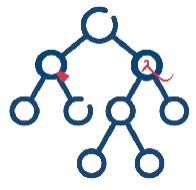
\includegraphics[height=1.0cm]{msca_logo.png}}%
    \end{center}

    \vspace{0.6cm}

    % Main title with Q logos on sides (with clickable links)
    \begin{center}
        \begin{minipage}{0.1\textwidth}
            \centering
            \href{https://quantlet.com}{
\includegraphics[height=1.1cm]{ql_logo.png}}
        \end{minipage}%
        \begin{minipage}{0.78\textwidth}
            \centering
            {\LARGE\bfseries\usebeamercolor[fg]{title}\inserttitle}

            \vspace{0.3cm}

            {\usebeamerfont{subtitle}\usebeamercolor[fg]{title}\insertsubtitle}
        \end{minipage}%
        \begin{minipage}{0.1\textwidth}
            \centering
            \href{https://quantinar.com}{
\includegraphics[height=1.1cm]{qr_logo.png}}
        \end{minipage}
    \end{center}

    \vspace{0.6cm}

    % Authors (left aligned)
    \hspace{0.5cm}{\usebeamerfont{author}\insertauthor}

    \vspace{0.3cm}

    % Institute/Affiliations (left aligned)
    \hspace{0.5cm}\begin{minipage}[t]{0.9\textwidth}
        \raggedright\small\insertinstitute
    \end{minipage}
}

%=============================================================================
% THEOREM ENVIRONMENTS
%=============================================================================
\theoremstyle{definition}
\setbeamertemplate{theorems}[numbered]
\ifdefined\tsalang
\newtheorem{defn}{Definiție}
\newtheorem{thm}{Teoremă}
\newtheorem{prop}{Propoziție}
\newtheorem{rmk}{Observație}
\else
\newtheorem{defn}{Definition}
\newtheorem{thm}{Theorem}
\newtheorem{prop}{Proposition}
\newtheorem{rmk}{Remark}
\fi

%=============================================================================
% CENTRED MINIPAGE (no extra vertical space)
%=============================================================================
\newenvironment{cminipage}[1]{%
    \par\noindent\hfill\begin{minipage}{#1}\ignorespaces
}{%
    \end{minipage}\hfill\null\par
}

%=============================================================================
% CUSTOM COMMANDS
%=============================================================================
\newcommand{\E}{\mathbb{E}}
\newcommand{\Var}{\text{Var}}
\newcommand{\Cov}{\text{Cov}}
\newcommand{\Corr}{\text{Corr}}
\newcommand{\R}{\mathbb{R}}
\newcommand{\N}{\mathbb{N}}
\newcommand{\Z}{\mathbb{Z}}
\newcommand{\B}{\mathbf{B}}
\newcommand{\imark}{\textcolor{MainBlue}{\textbullet}}
\newcommand{\RMSE}{\text{RMSE}}
\newcommand{\MAE}{\text{MAE}}
\newcommand{\MAPE}{\text{MAPE}}

% Boldface vector/matrix commands (VAR, VECM, state space; also used by the older TSA decks)
\newcommand{\bY}{\mathbf{Y}}
\newcommand{\bX}{\mathbf{X}}
\newcommand{\bA}{\mathbf{A}}
\newcommand{\bB}{\mathbf{B}}
\newcommand{\bepsilon}{\boldsymbol{\varepsilon}}
\newcommand{\bSigma}{\boldsymbol{\Sigma}}
\newcommand{\bPhi}{\boldsymbol{\Phi}}
\newcommand{\bGamma}{\boldsymbol{\Gamma}}
\newcommand{\bPi}{\boldsymbol{\Pi}}
\newcommand{\bc}{\mathbf{c}}
\newcommand{\balpha}{\boldsymbol{\alpha}}
\newcommand{\bbeta}{\boldsymbol{\beta}}
\newcommand{\bvarepsilon}{\boldsymbol{\varepsilon}}

% Legacy seminar marks (older TSA seminar decks)
\newcommand{\correct}{\textcolor{Forest}{\checkmark}}
\newcommand{\incorrect}{\textcolor{Crimson}{\texttimes}}
 se definește
%   \newcommand{\coursename}{Time Series Analysis}      (EN)
%   \newcommand{\coursename}{Serii de timp}       (RO)  și  \def\tsalang{ro}
% Fișierele .tex se află în EN/Courses, EN/Seminars, RO/Cursuri, RO/Seminarii (două niveluri sub rădăcină).
% Deck-urile sînt generate de latex/build_chapterN.py / build_seminarN.py (vezi latex/tsa_build.py).

\documentclass[9pt, aspectratio=169, t]{beamer}
\providecommand{\coursename}{Time Series Analysis}

% Ensure content fits on slides
\setbeamersize{text margin left=8mm, text margin right=8mm}
% Smaller institute font (title page)
\setbeamerfont{institute}{size=\footnotesize}

%=============================================================================
% THEME AND STYLE CONFIGURATION
%=============================================================================
\usetheme{default}
% Using default theme for clean header/footer control

% Color Palette (matching Redispatch PDF)
\definecolor{MainBlue}{RGB}{26, 58, 110}
\definecolor{AccentBlue}{RGB}{26, 58, 110}
\definecolor{IDAred}{RGB}{205, 0, 0}
\definecolor{DarkGray}{RGB}{51, 51, 51}
\definecolor{MediumGray}{RGB}{128, 128, 128}
\definecolor{LightGray}{RGB}{248, 248, 248}
\definecolor{VeryLightGray}{RGB}{235, 235, 235}
\definecolor{KeynoteGray}{RGB}{218, 218, 218}
\definecolor{SectionGray}{RGB}{120, 120, 120}
\definecolor{FooterGray}{RGB}{100, 100, 100}
\definecolor{Crimson}{RGB}{220, 53, 69}
\definecolor{Forest}{RGB}{46, 125, 50}
\definecolor{Amber}{RGB}{181, 133, 63}
\definecolor{Orange}{RGB}{230, 126, 34}
\definecolor{Purple}{RGB}{142, 68, 173}

% Gradient background (exact Keynote 315° gradient: white to RGB 218,218,218)
\setbeamertemplate{background}{%
    \begin{tikzpicture}[remember picture, overlay]
        \shade[shading=axis, shading angle=315,
        top color=white, bottom color=KeynoteGray]
        (current page.south west) rectangle (current page.north east);
    \end{tikzpicture}%
}
% Fallback solid color for compatibility
\setbeamercolor{background canvas}{bg=}

\setbeamercolor{palette primary}{bg=MainBlue, fg=white}
\setbeamercolor{palette secondary}{bg=MainBlue!85, fg=white}
\setbeamercolor{palette tertiary}{bg=MainBlue!70, fg=white}
\setbeamercolor{structure}{fg=MainBlue}
\setbeamercolor{title}{fg=IDAred}
\setbeamercolor{frametitle}{fg=IDAred, bg=}
\setbeamercolor{block title}{bg=MainBlue, fg=white}
\setbeamercolor{block body}{bg=VeryLightGray, fg=DarkGray}
\setbeamercolor{block title alerted}{bg=Crimson, fg=white}
\setbeamercolor{block body alerted}{bg=Crimson!8, fg=DarkGray}
\setbeamercolor{block title example}{bg=Forest, fg=white}
\setbeamercolor{block body example}{bg=Forest!8, fg=DarkGray}
\setbeamercolor{item}{fg=MainBlue}

% Footer colors (override Madrid theme blue)
\setbeamercolor{author in head/foot}{fg=FooterGray, bg=}
\setbeamercolor{title in head/foot}{fg=FooterGray, bg=}
\setbeamercolor{date in head/foot}{fg=FooterGray, bg=}
\setbeamercolor{section in head/foot}{fg=FooterGray, bg=}
\setbeamercolor{subsection in head/foot}{fg=FooterGray, bg=}

% Bullet styles (apply everywhere including blocks)
\setbeamertemplate{itemize item}{\color{MainBlue}$\boxdot$}
\setbeamertemplate{itemize subitem}{\color{MainBlue}$\blacktriangleright$}
\setbeamertemplate{itemize subsubitem}{\color{MainBlue}\tiny$\bullet$}
\setbeamertemplate{itemize/enumerate body begin}{\normalsize}
\setbeamertemplate{itemize/enumerate subbody begin}{\normalsize}

% Item spacing - compact style
\setlength{\leftmargini}{10pt}       % Level 1: minimal indent
\setlength{\leftmarginii}{10pt}      % Level 2: minimal additional indent
% Compact list spacing (zero extra space before/after lists in blocks)
\makeatletter
\def\@listi{\leftmargin\leftmargini \topsep 0pt \parsep 0pt \itemsep 0pt}
\def\@listii{\leftmargin\leftmarginii \topsep 0pt \parsep 0pt \itemsep 0pt}
\makeatother

\setbeamertemplate{navigation symbols}{}

%=============================================================================
% CUSTOM HEADLINE
%=============================================================================
\setbeamertemplate{headline}{%
    \vskip10pt%
    \hbox to \paperwidth{%
        \hskip0.5cm%
        {\small\color{FooterGray}\renewcommand{\hyperlink}[2]{##2}\insertsectionhead}%
        \hfill%
        \textcolor{FooterGray}{\small\insertframenumber}%
        \hskip0.5cm%
    }%
    \vskip4pt%
    {\color{FooterGray}\hrule height 0.4pt}%
}

%=============================================================================
% CUSTOM FOOTER
%=============================================================================
\usepackage{fontawesome5}

\setbeamertemplate{footline}{%
    {\color{FooterGray}\hrule height 0.4pt}%
    \vskip4pt%
    \hbox to \paperwidth{%
        \hskip0.5cm%
        \textcolor{FooterGray}{\small\coursename}%
        \hfill%
        \raisebox{-0.1em}{%
            \begin{tikzpicture}[x=0.08em, y=0.08em, line width=0.4pt]
                \draw[FooterGray] (0,3) -- (1,4) -- (2,3.5) -- (3,5) -- (4,4) -- (5,6) -- (6,5.5) -- (7,4) -- (8,5) -- (9,7) -- (10,6) -- (11,5) -- (12,6.5) -- (13,8) -- (14,7) -- (15,6) -- (16,7.5) -- (17,9) -- (18,8) -- (19,7) -- (20,8.5) -- (21,10) -- (22,9) -- (23,8) -- (24,9.5);
            \end{tikzpicture}%
        }%
        \hskip0.5cm%
    }%
    \vskip6pt%
}

%=============================================================================
% PACKAGES
%=============================================================================
\usepackage[utf8]{inputenc}
\DeclareUnicodeCharacter{03B1}{\ensuremath{\alpha}}
\usepackage[T1]{fontenc}
\usepackage{amsmath, amssymb, amsthm}
\usepackage{mathtools}
\usepackage{bm}
\usepackage{tikz}
\usetikzlibrary{arrows.meta, positioning, shapes, calc, decorations.pathreplacing, shadings}
\usepackage{booktabs}
\usepackage{multirow}
\usepackage{array}
\usepackage{graphicx}
\usepackage{animate}
\usepackage{hyperref}
\usepackage{colortbl}
\usepackage{listings}
\lstset{language=Python, basicstyle=\ttfamily\scriptsize, keywordstyle=\color{MainBlue}\bfseries,
  commentstyle=\color{Forest}, stringstyle=\color{Crimson}, breaklines=true,
  frame=none, backgroundcolor=\color{VeryLightGray}, xleftmargin=2mm}
\hypersetup{colorlinks=true, linkcolor=MainBlue, urlcolor=MainBlue}
\graphicspath{{../../logos/}{../../charts/}{../../photos/}}
\usepackage{xcolor}
\hfuzz=2pt  % Suppress tiny overfull warnings (<2pt)
\vfuzz=2pt  % Suppress tiny vertical overfull warnings (<2pt)
% \mathrm in the sans-serif family of the slides (beamer resets \mathrm to the serif family at \begin{document};
% this hook runs after beamer's, so WN, Var, RMSE, ... in formulas match the surrounding text)
% Bold vectors and matrices in the same sans-serif family: \mathbf{A} in sans bold (beamer's own \mathbf came out in
% medium weight), and the bold upright Greek capitals of \boldsymbol / \bm (\bSigma, \bPhi, \boldsymbol{\Theta}) in
% cmss bold: bm.sty fixes its "boldoperators" font when it is loaded (serif cmbx), before beamer switches the
% operators to cmss, so it is reset here.
\AtBeginDocument{%
  \SetMathAlphabet{\mathrm}{normal}{\encodingdefault}{\sfdefault}{\mddefault}{n}%
  \SetMathAlphabet{\mathrm}{bold}{\encodingdefault}{\sfdefault}{bx}{n}%
  \SetMathAlphabet{\mathbf}{normal}{\encodingdefault}{\sfdefault}{bx}{n}%
  \SetMathAlphabet{\mathbf}{bold}{\encodingdefault}{\sfdefault}{bx}{n}%
  \SetSymbolFont{boldoperators}{normal}{OT1}{cmss}{bx}{n}%
  \SetSymbolFont{boldoperators}{bold}{OT1}{cmss}{bx}{n}}

%=============================================================================
% QUANTLET COMMANDS
%   \quantlet{<displayed name>}{<url>}       (generic, compatible with the older TSA decks)
%   \tsaquantlet{Ch_05}{TSA_ch5_garch}       -> https://github.com/danpele/Time-Series-Analysis/tree/main/Quantlets/Ch_05/TSA_ch5_garch
%   \qlurl{<folder>} is defined per chapter by the generator (Quantlets/Ch_NN/<folder>)
%=============================================================================
\newcommand{\tsarepo}{https://github.com/danpele/Time-Series-Analysis}
\newcommand{\tsaqlbase}{https://github.com/danpele/Time-Series-Analysis/tree/main/Quantlets}
\newcommand{\quantlet}[2]{%
    \hfill\href{#2}{%
        \raisebox{-0.15em}{
\includegraphics[height=0.7em]{ql_logo.png}}%
        \textcolor{MainBlue}{\tiny\ #1}%
    }%
}
\newcommand{\tsaquantlet}[2]{\quantlet{\detokenize{#2}}{\tsaqlbase/#1/#2}}

%=============================================================================
% NOTEBOOKS (Google Colab)
%   \colaburl{notebooks/EN/chapter5_seminar_notebook.ipynb} -> the Colab link of a file in the TSA repo
%   \nb: the chapter notebook (each seminar deck redefines it with \renewcommand)
%=============================================================================
\newcommand{\colaburl}[1]{https://colab.research.google.com/github/danpele/Time-Series-Analysis/blob/main/#1}
\newcommand{\nb}{https://colab.research.google.com/github/danpele/Time-Series-Analysis/tree/main/notebooks/EN}
\newcommand{\nbname}{notebooks/EN}

%=============================================================================
% SLIDE HELPERS (used by the generators; the same as in MFM)
%=============================================================================
% local font size for list bodies (the preamble forces \normalsize)
\newcommand{\itemsize}[1]{\setbeamertemplate{itemize/enumerate body begin}{#1}\setbeamertemplate{itemize/enumerate subbody begin}{#1}}
\newcommand{\intitle}[1]{{\hypersetup{urlcolor=white}#1}}   % white links inside coloured title bars
\newcommand{\imgcap}[1]{{\scriptsize #1}\\[0.5mm]}          % caption under a photo
\newcommand{\imgcredit}[2]{{\tiny\color{FooterGray}\href{#1}{#2}}}   % image credit: source URL, author/licence
\newcommand{\aiprompt}[1]{{\ttfamily\color{MainBlue}#1}}     % a prompt to an AI assistant

%=============================================================================
% SEMINARS: student version by default; the instructor wrapper *_solutions.tex sets \solutionstrue
%=============================================================================
\makeatletter\@ifundefined{ifsolutions}{\expandafter\newif\csname ifsolutions\endcsname}{}\makeatother
\newcommand{\solonly}[1]{\ifsolutions #1\fi}
\newcommand{\propsub}{\ifsolutions\else\framesubtitle{\ifdefined\tsalang Rezolvarea se discută la seminar\else Solution discussed in class\fi}\fi}

%=============================================================================
% APPENDIX AND CHAPTER LINKS (latex/appendix_links.py writes the calls; it also re-declares these
% macros before \begin{document}, so the decks compile with or without this preamble block)
%=============================================================================
\providecommand{\tsaapplink}[3]{\hypertarget{#2}{}\hyperlink{#1}{\beamergotobutton{#3}}}
\providecommand{\tsaappback}[2]{\begin{tikzpicture}[remember picture,overlay]\node[anchor=south east] at ([xshift=-3mm,yshift=7mm]current page.south east){\hyperlink{#1}{\beamerreturnbutton{#2}}};\end{tikzpicture}}
\providecommand{\tsachlink}[2]{\href{#1}{#2}}
\providecommand{\tsachlinkt}[2]{\href{#1}{\usebeamercolor[fg]{frametitle}#2}}

%=============================================================================
% QUANTINAR COMMAND: link către un curs Quantinar (subiecte avansate)
%=============================================================================
\newcommand{\quantinar}[2]{%
    \href{#2}{%
        \raisebox{-0.15em}{
\includegraphics[height=0.8em]{qr_logo.png}}%
        \textcolor{MainBlue}{\scriptsize\ #1}%
    }%
}

%=============================================================================
% CUSTOM TITLE PAGE
%=============================================================================
\defbeamertemplate*{title page}{hybrid}[1][]
{
    \vspace{0.2cm}
    % Logos row - top header (with clickable links)
    \begin{center}
        \href{https://www.ase.ro}{
\includegraphics[height=1.0cm]{ase_logo.png}}\hspace{0.3cm}%
        \href{https://theida.net}{
\includegraphics[height=1.0cm]{ida_logo.png}}\hspace{0.3cm}%
        \href{https://blockchain-research-center.com}{
\includegraphics[height=1.0cm]{brc_logo.png}}\hspace{0.3cm}%
        \href{https://www.ai4efin.ase.ro}{
\includegraphics[height=1.0cm]{ai4efin_logo.png}}\hspace{0.3cm}%
        \href{https://ipe.ro/new}{
\includegraphics[height=1.0cm]{acad_logo.png}}\hspace{0.3cm}%
        \href{https://www.digital-finance-msca.com}{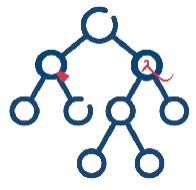
\includegraphics[height=1.0cm]{msca_logo.png}}%
    \end{center}

    \vspace{0.6cm}

    % Main title with Q logos on sides (with clickable links)
    \begin{center}
        \begin{minipage}{0.1\textwidth}
            \centering
            \href{https://quantlet.com}{
\includegraphics[height=1.1cm]{ql_logo.png}}
        \end{minipage}%
        \begin{minipage}{0.78\textwidth}
            \centering
            {\LARGE\bfseries\usebeamercolor[fg]{title}\inserttitle}

            \vspace{0.3cm}

            {\usebeamerfont{subtitle}\usebeamercolor[fg]{title}\insertsubtitle}
        \end{minipage}%
        \begin{minipage}{0.1\textwidth}
            \centering
            \href{https://quantinar.com}{
\includegraphics[height=1.1cm]{qr_logo.png}}
        \end{minipage}
    \end{center}

    \vspace{0.6cm}

    % Authors (left aligned)
    \hspace{0.5cm}{\usebeamerfont{author}\insertauthor}

    \vspace{0.3cm}

    % Institute/Affiliations (left aligned)
    \hspace{0.5cm}\begin{minipage}[t]{0.9\textwidth}
        \raggedright\small\insertinstitute
    \end{minipage}
}

%=============================================================================
% THEOREM ENVIRONMENTS
%=============================================================================
\theoremstyle{definition}
\setbeamertemplate{theorems}[numbered]
\ifdefined\tsalang
\newtheorem{defn}{Definiție}
\newtheorem{thm}{Teoremă}
\newtheorem{prop}{Propoziție}
\newtheorem{rmk}{Observație}
\else
\newtheorem{defn}{Definition}
\newtheorem{thm}{Theorem}
\newtheorem{prop}{Proposition}
\newtheorem{rmk}{Remark}
\fi

%=============================================================================
% CENTRED MINIPAGE (no extra vertical space)
%=============================================================================
\newenvironment{cminipage}[1]{%
    \par\noindent\hfill\begin{minipage}{#1}\ignorespaces
}{%
    \end{minipage}\hfill\null\par
}

%=============================================================================
% CUSTOM COMMANDS
%=============================================================================
\newcommand{\E}{\mathbb{E}}
\newcommand{\Var}{\text{Var}}
\newcommand{\Cov}{\text{Cov}}
\newcommand{\Corr}{\text{Corr}}
\newcommand{\R}{\mathbb{R}}
\newcommand{\N}{\mathbb{N}}
\newcommand{\Z}{\mathbb{Z}}
\newcommand{\B}{\mathbf{B}}
\newcommand{\imark}{\textcolor{MainBlue}{\textbullet}}
\newcommand{\RMSE}{\text{RMSE}}
\newcommand{\MAE}{\text{MAE}}
\newcommand{\MAPE}{\text{MAPE}}

% Boldface vector/matrix commands (VAR, VECM, state space; also used by the older TSA decks)
\newcommand{\bY}{\mathbf{Y}}
\newcommand{\bX}{\mathbf{X}}
\newcommand{\bA}{\mathbf{A}}
\newcommand{\bB}{\mathbf{B}}
\newcommand{\bepsilon}{\boldsymbol{\varepsilon}}
\newcommand{\bSigma}{\boldsymbol{\Sigma}}
\newcommand{\bPhi}{\boldsymbol{\Phi}}
\newcommand{\bGamma}{\boldsymbol{\Gamma}}
\newcommand{\bPi}{\boldsymbol{\Pi}}
\newcommand{\bc}{\mathbf{c}}
\newcommand{\balpha}{\boldsymbol{\alpha}}
\newcommand{\bbeta}{\boldsymbol{\beta}}
\newcommand{\bvarepsilon}{\boldsymbol{\varepsilon}}

% Legacy seminar marks (older TSA seminar decks)
\newcommand{\correct}{\textcolor{Forest}{\checkmark}}
\newcommand{\incorrect}{\textcolor{Crimson}{\texttimes}}


\newcommand{\qlurl}[1]{https://github.com/danpele/Time-Series-Analysis/tree/main/Quantlets/Ch_06/#1}
\renewcommand{\nb}{\colaburl{notebooks/EN/chapter6_seminar_notebook.ipynb}}
\renewcommand{\nbname}{chapter6\_seminar\_notebook.ipynb}
% left column: full width in the student version, narrower next to the solution
\newcommand{\taskw}{\ifsolutions 0.47\textwidth\else 0.96\textwidth\fi}
\newcommand{\solw}{\ifsolutions 0.49\textwidth\else 0pt\fi}

% Clickable citations (DOIs verified via Crossref)
\newcommand{\refHP}{\href{https://doi.org/10.1007/978-3-031-13584-2}{Huang and Petukhina (2022)}}
\newcommand{\refFPP}{\href{https://otexts.com/fpp3/VAR.html}{Hyndman and Athanasopoulos (2021)}}
\newcommand{\refLut}{\href{https://doi.org/10.1007/978-3-540-27752-1}{Lütkepohl (2005)}}
\newcommand{\refHamilton}{\href{https://doi.org/10.2307/j.ctv14jx6sm}{Hamilton (1994)}}
\newcommand{\refSims}{\href{https://doi.org/10.2307/1912017}{Sims (1980)}}
\newcommand{\refSimsPP}{\href{https://doi.org/10.1016/0014-2921(92)90041-T}{Sims (1992)}}
\newcommand{\refGranger}{\href{https://doi.org/10.2307/1912791}{Granger (1969)}}
\newcommand{\refLutOm}{\href{https://doi.org/10.1016/0304-4076(82)90011-2}{Lütkepohl (1982)}}
\newcommand{\refTY}{\href{https://doi.org/10.1016/0304-4076(94)01616-8}{Toda and Yamamoto (1995)}}
\newcommand{\refSSW}{\href{https://doi.org/10.2307/2938337}{Sims, Stock and Watson (1990)}}
\newcommand{\refSW}{\href{https://doi.org/10.1257/jep.15.4.101}{Stock and Watson (2001)}}
\newcommand{\refPS}{\href{https://doi.org/10.1016/S0165-1765(97)00214-0}{Pesaran and Shin (1998)}}
\newcommand{\refKPP}{\href{https://doi.org/10.1016/0304-4076(95)01753-4}{Koop, Pesaran and Potter (1996)}}
\newcommand{\refDY}{\href{https://doi.org/10.1111/j.1468-0297.2008.02208.x}{Diebold and Yilmaz (2009)}}
\newcommand{\refDYb}{\href{https://doi.org/10.1016/j.ijforecast.2011.02.006}{Diebold and Yilmaz (2012)}}
\newcommand{\refKilian}{\href{https://doi.org/10.1162/003465398557465}{Kilian (1998)}}
\newcommand{\refHosking}{\href{https://doi.org/10.1080/01621459.1980.10477520}{Hosking (1980)}}
\newcommand{\refJB}{\href{https://doi.org/10.1016/0165-1765(80)90024-5}{Jarque and Bera (1980)}}
\newcommand{\refAkaike}{\href{https://doi.org/10.1109/TAC.1974.1100705}{Akaike (1974)}}
\newcommand{\refSchwarz}{\href{https://doi.org/10.1214/aos/1176344136}{Schwarz (1978)}}
\newcommand{\refHQ}{\href{https://doi.org/10.1111/j.2517-6161.1979.tb01072.x}{Hannan and Quinn (1979)}}
\newcommand{\refDM}{\href{https://doi.org/10.1080/07350015.1995.10524599}{Diebold and Mariano (1995)}}
\newcommand{\refEG}{\href{https://doi.org/10.2307/1913236}{Engle and Granger (1987)}}

\title[Time Series Analysis]{Time Series Analysis}
\subtitle{Seminar 6: VAR models and Granger causality\ifsolutions\ (instructor version)\fi}
\author[D.T. Pele]{Daniel Traian PELE}
\institute{Bucharest University of Economic Studies\\
IDA Institute Digital Assets\\
Blockchain Research Center\\
AI4EFin Artificial Intelligence for Energy Finance\\
Romanian Academy, Institute for Economic Forecasting\\
MSCA Digital Finance}
\date{}

%=============================================================================
\providecommand{\tsaapplink}[3]{\hypertarget{#2}{}\hyperlink{#1}{\beamergotobutton{#3}}}  % APPLINKS-MACROS
\providecommand{\tsaappback}[2]{\begin{tikzpicture}[remember picture,overlay]\node[anchor=south east] at ([xshift=-3mm,yshift=7mm]current page.south east){\hyperlink{#1}{\beamerreturnbutton{#2}}};\end{tikzpicture}}  % APPLINKS-MACROS
\providecommand{\tsachlink}[2]{\href{#1}{#2}}  % APPLINKS-MACROS
\providecommand{\tsachlinkt}[2]{\href{#1}{\usebeamercolor[fg]{frametitle}#2}}  % APPLINKS-MACROS
\begin{document}
%=============================================================================

{
\setbeamertemplate{headline}{}
\setbeamertemplate{footline}{}
\begin{frame}[noframenumbering]
    \titlepage
\end{frame}
}
% BEGIN-ACRONYMS (generat de latex/acronyms.py; nu editati manual)
\begin{frame}{Acronyms used in this material}
\setbeamertemplate{itemize/enumerate body begin}{\tiny}
\begin{columns}[T]
\begin{column}{0.49\textwidth}
\begin{itemize}\setlength{\itemsep}{0pt}
    \item \textbf{AI}: Artificial Intelligence
    \item \textbf{AIC}: Akaike Information Criterion
    \item \textbf{BET}: Bucharest Exchange Trading (index)
    \item \textbf{BIC}: Bayesian Information Criterion
    \item \textbf{BNR}: Banca Națională a României (the National Bank of Romania)
    \item \textbf{CCF}: Cross-Correlation Function
    \item \textbf{EODHD}: EOD Historical Data (market-data provider)
    \item \textbf{FEVD}: Forecast Error Variance Decomposition
    \item \textbf{GDP}: Gross Domestic Product
    \item \textbf{HICP}: Harmonised Index of Consumer Prices
    \item \textbf{HQ}: Hannan–Quinn (information criterion)
    \item \textbf{OLS}: Ordinary Least Squares
    \item \textbf{ROBOR}: Romanian Interbank Offer Rate
\end{itemize}
\end{column}
\begin{column}{0.49\textwidth}
\begin{itemize}\setlength{\itemsep}{0pt}
    \item \textbf{SE}: Standard Error
    \item \textbf{VAR}: Vector AutoRegression
\end{itemize}
\end{column}
\end{columns}
\end{frame}
% END-ACRONYMS

\begin{frame}{Today's question and route}
\itemsize{\small}
\begin{itemize}
    \item \textbf{Question}: when we model several series together, which of them helps to forecast the others, and how does a shock in one spread to the rest?
    \begin{itemize}
        \item this seminar comes \textbf{before} Lecture 6: the section ``What you need today'' gives every definition the tasks use
    \end{itemize}
    \item Route
    \begin{itemize}
        \item Part A: a VAR(1) by hand (stability, mean, forecasts); impulse responses with the Cholesky factor; a variance decomposition; a Granger $F$ test; lag selection
        \item Part B: does the S\&P 500 lead the BET (daily and weekly)? a VAR for Romanian GDP growth, inflation and ROBOR 3M; the EUR/RON rate added to it
        \item Part C: an open question on the ``price puzzle'' and an AI answer to audit
    \end{itemize}
    \item Notebook for today: \href{\nb}{open the seminar notebook in Google Colab}; each task names its notebook section
\end{itemize}
\end{frame}

\begin{frame}{Exercise map}
\itemsize{\small}
\begin{center}
\footnotesize
\begin{tabular}{>{\raggedright\arraybackslash}p{1.1cm}>{\raggedright\arraybackslash}p{7.5cm}>{\raggedright\arraybackslash}p{1.9cm}>{\raggedright\arraybackslash}p{1.4cm}}
\toprule
\textbf{Task} & \textbf{Question} & \textbf{Type} & \textbf{Model} \\
\midrule
A1, A2 & a VAR(1) by hand: stability, mean, forecasts & Solved, Proposed & A1 \\
A3, A4 & orthogonalised impulse responses; a variance decomposition & Solved, Proposed & A3 \\
A5, A6 & a Granger $F$ test; lag selection by AIC, BIC and HQ & Solved, Proposed & A5 \\
B1, B2 & S\&P 500 and BET: daily; weekly & Solved, Proposed & B1 \\
B3, B4 & a Romanian macro VAR; the EUR/RON rate added & Solved, Proposed & B3 \\
C1, C2 & the price puzzle; what is wrong in an AI answer? & Proposed & B3 \\
\bottomrule
\end{tabular}
\end{center}
\begin{itemize}
    \item \textbf{[Solved]}: full solution in the slides and in the notebook, a model to follow; \textbf{[Proposed]}: you solve it, following the model
\end{itemize}
\end{frame}

\begin{frame}{Data used}
\itemsize{\small}
\begin{center}
\footnotesize
\begin{tabular}{llll}
\toprule
\textbf{Series} & \textbf{Source} & \textbf{Frequency} & \textbf{Period} \\
\midrule
S\&P 500, BET & EODHD & daily, close & 2000--2026 \\
Real GDP, Romania & Eurostat (namq\_10\_gdp) & quarterly, seasonally adjusted & 2005--2026 \\
HICP, Romania & Eurostat (prc\_hicp\_minr) & monthly, 2015 = 100 & 2004--2026 \\
ROBOR 3M & Eurostat (irt\_st\_m) & monthly, \% per year & 2005--2026 \\
EUR/RON & BNR reference rate & daily & 2005--2026 \\
\bottomrule
\end{tabular}
\end{center}
\begin{itemize}
    \item Quarterly VAR variables: $g_t = 100\Delta\ln\mathrm{GDP}_t$; $\pi_t$: 12-month HICP inflation (quarterly mean); $i_t$: ROBOR 3M (quarterly mean); $s_t$: $100\Delta\ln$ of the quarterly mean EUR/RON
    \item In the notebook: \texttt{VAR} from \texttt{statsmodels}, \texttt{granger\_F}, \texttt{ic\_table}, \texttt{girf}; no account or key is needed
\end{itemize}
\end{frame}


%=============================================================================
\section{What you need today}
%=============================================================================

\begin{frame}{What you need today (1/4): the VAR model and its stability}
\itemsize{\small}
\begin{itemize}
    \item \textbf{VAR$(p)$}: $\bY_t = \bc + \bA_1\bY_{t-1} + \dots + \bA_p\bY_{t-p} + \bepsilon_t$; $\bY_t$: $K$ series; $\bA_j$: $K \times K$; $\bepsilon_t$ white noise, $E[\bepsilon_t\bepsilon_t'] = \bSigma$
    \begin{itemize}
        \item equation by equation: each variable is regressed on a constant and the $p$ lags of all variables; $a_{jk}$: effect of $y_{k,t-1}$ on $y_{jt}$
    \end{itemize}
    \item \textbf{Stability} of a VAR(1): all eigenvalues of $\bA$ have $|\lambda| < 1$; for $K = 2$: $\lambda^2 - \mathrm{tr}(\bA)\lambda + \det(\bA) = 0$
    \begin{itemize}
        \item complex $\lambda = a \pm bi$: modulus $\sqrt{a^2 + b^2}$; VAR$(p)$: the eigenvalues of the companion matrix $\begin{pmatrix} \bA_1 & \bA_2 \\ \mathbf{I} & \mathbf{0} \end{pmatrix}$ (for $p = 2$)
    \end{itemize}
    \item \textbf{Mean} of a stable VAR(1): $\boldsymbol{\mu} = (\mathbf{I} - \bA)^{-1}\bc$; \textbf{forecasts}: $\hat\bY_{T+1} = \bc + \bA\bY_T$, $\hat\bY_{T+2} = \bc + \bA\hat\bY_{T+1}$
    \begin{itemize}
        \item inverse of a $2 \times 2$ matrix: $\begin{pmatrix} a & b \\ c & d \end{pmatrix}^{-1} = \frac{1}{ad - bc}\begin{pmatrix} d & -b \\ -c & a \end{pmatrix}$
    \end{itemize}
\end{itemize}
\end{frame}

\begin{frame}{What you need today (2/4): estimation, lag order and diagnostics}
\itemsize{\small}
\begin{itemize}
    \item \textbf{Estimation}: OLS equation by equation (all equations have the same regressors); $K + pK^2$ coefficients
    \begin{itemize}
        \item the variables must be stationary (\tsachlink{https://danpele.github.io/Time-Series-Analysis/EN/Courses/chapter3_unit_roots_arima_models.pdf}{Chapter 3}): growth rates, returns, or rates that do not trend
    \end{itemize}
    \item \textbf{Lag order}: $\mathrm{IC}(p) = \ln\det\tilde\bSigma(p) + c_T\,pK^2/T$, smallest is best, on a common sample
    \begin{itemize}
        \item $c_T = 2$ (AIC), $\ln T$ (BIC), $2\ln\ln T$ (HQ); BIC chooses the smallest $p$, AIC the largest
    \end{itemize}
    \item \textbf{Portmanteau test}: $H_0$: residuals without auto- and cross-correlation up to lag $h$; $Q_h \sim \chi^2(K^2(h - p))$
    \begin{itemize}
        \item a small p-value: add lags or variables; normality (Jarque--Bera) often fails because of crises
    \end{itemize}
\end{itemize}
\end{frame}

\begin{frame}{What you need today (3/4): Granger causality}
\itemsize{\small}
\begin{itemize}
    \item $x$ \textbf{Granger-causes} $y$ if the past of $x$ improves the forecast of $y$ beyond the past of $y$ and of the other variables
    \begin{itemize}
        \item in a VAR$(p)$: $H_0$: the $p$ coefficients of $x_{t-1}, \dots, x_{t-p}$ in the equation of $y$ are all zero
    \end{itemize}
    \item \textbf{$F$ test}: $F = \dfrac{(RSS_R - RSS_U)/q}{RSS_U/(T - k)}$; $q$: number of restrictions; $k$: coefficients of the unrestricted equation
    \begin{itemize}
        \item reject $H_0$ if $F$ exceeds the critical value of $F(q, T - k)$ (about 3.1 for $q = 2$ and $T - k \approx 80$--100)
    \end{itemize}
    \item \textbf{Not} cause and effect: a statement about predictability, relative to the chosen variables
    \begin{itemize}
        \item pitfalls: an omitted common driver; effects within the same period (instantaneous causality, in $\bSigma$); non-stationary series
    \end{itemize}
\end{itemize}
\end{frame}

\begin{frame}{What you need today (4/4): impulse responses and FEVD}
\itemsize{\small}
\begin{itemize}
    \item \textbf{Impulse responses} of a VAR(1): $\bPhi_h = \bA^h$; column $k$: the path of all variables after a unit shock to $\varepsilon_k$
    \begin{itemize}
        \item the shocks are correlated, so we use $\bSigma = \mathbf{P}\mathbf{P}'$ (\textbf{Cholesky}, $\mathbf{P}$ lower triangular) and $\boldsymbol{\Theta}_h = \bPhi_h\mathbf{P}$
        \item $2 \times 2$: $p_{11} = \sqrt{\sigma_{11}}$, $p_{21} = \sigma_{21}/p_{11}$, $p_{22} = \sqrt{\sigma_{22} - p_{21}^2}$
    \end{itemize}
    \item \textbf{The ordering matters}: the first variable does not react within the period to the shocks of the others
    \begin{itemize}
        \item the \textbf{generalised} responses \refPS\ do not depend on the order: $\bPhi_h\bSigma\mathbf{e}_k/\sqrt{\sigma_{kk}}$
    \end{itemize}
    \item \textbf{FEVD}: share of shock $k$ in the $h$-step forecast error variance of $y_j$: $\sum_{s<h}\theta_{jk,s}^2 / \sum_{s<h}\sum_m\theta_{jm,s}^2$
    \begin{itemize}
        \item each row sums to 100\%
    \end{itemize}
\end{itemize}
\end{frame}


%=============================================================================
\section{Part A: computations on paper}
%=============================================================================

\begin{frame}{A1: a VAR(1) by hand [Solved]}
\itemsize{\scriptsize}
\begin{columns}[T]
\begin{column}{0.47\textwidth}
\begin{block}{Task}
\begin{itemize}
    \item $\bc = (0.4, 0.8)'$, $\bA = \begin{pmatrix} 0.6 & 0.2 \\ 0.2 & 0.6 \end{pmatrix}$; last observation $\bY_T = (3, 2)'$.
    \item 1. Write the two equations.
    \item 2. Find the eigenvalues of $\bA$ and decide whether the VAR is stable.
    \item 3. Compute the mean $\boldsymbol{\mu}$.
    \item 4. Compute $\hat\bY_{T+1}$ and $\hat\bY_{T+2}$.
    \item Report: two equations, two eigenvalues, $\boldsymbol{\mu}$, two forecasts.
\end{itemize}
\end{block}
\end{column}
\begin{column}{0.49\textwidth}
\begin{exampleblock}{Solution}
\begin{itemize}
    \item 1. $y_{1t} = 0.4 + 0.6y_{1,t-1} + 0.2y_{2,t-1} + \varepsilon_{1t}$; $y_{2t} = 0.8 + 0.2y_{1,t-1} + 0.6y_{2,t-1} + \varepsilon_{2t}$
    \item 2. $\mathrm{tr} = 1.2$, $\det = 0.36 - 0.04 = 0.32$: $\lambda^2 - 1.2\lambda + 0.32 = 0$, $\lambda = 0.8$ and $0.4$; both below 1: stable
    \item 3. $\mathbf{I} - \bA = \begin{pmatrix} 0.4 & -0.2 \\ -0.2 & 0.4 \end{pmatrix}$, $\det = 0.12$; $\boldsymbol{\mu} = \frac{1}{0.12}\begin{pmatrix} 0.4 & 0.2 \\ 0.2 & 0.4 \end{pmatrix}\begin{pmatrix} 0.4 \\ 0.8 \end{pmatrix} = \begin{pmatrix} 2.667 \\ 3.333 \end{pmatrix}$
    \item 4. $\hat\bY_{T+1} = (0.4 + 1.8 + 0.4,\ 0.8 + 0.6 + 1.2)' = \begin{pmatrix} 2.60 \\ 2.60 \end{pmatrix}$; $\hat\bY_{T+2} = \begin{pmatrix} 2.48 \\ 2.88 \end{pmatrix}$: moving towards $\boldsymbol{\mu}$
\end{itemize}
\end{exampleblock}
\end{column}
\end{columns}
\end{frame}

\begin{frame}{A2: stable or not? [Proposed]}
\propsub
\itemsize{\scriptsize}
\begin{columns}[T]
\begin{column}{\taskw}
\begin{block}{Task}
\begin{itemize}
    \item Two VAR(1) matrices: (a) $\bA = \begin{pmatrix} 0.9 & 0.3 \\ 0.2 & 0.8 \end{pmatrix}$; (b) $\bA = \begin{pmatrix} 0.5 & -0.4 \\ 0.4 & 0.5 \end{pmatrix}$. Model: A1.
    \item 1. For each matrix, compute the trace, the determinant and the eigenvalues.
    \item 2. Decide whether each VAR is stable.
    \item 3. Describe how the responses to a shock behave in each case.
    \item Report: four eigenvalues (or moduli), two decisions and two sentences.
\end{itemize}
\end{block}
\end{column}
\begin{column}{\solw}
\solonly{%
\begin{exampleblock}{Solution}
\begin{itemize}
    \item 1. (a) $\mathrm{tr} = 1.7$, $\det = 0.66$: $\lambda = 1.1$, $0.6$; (b) $\mathrm{tr} = 1$, $\det = 0.41$: $\lambda = 0.5 \pm 0.4i$, $|\lambda| = 0.640$
    \item 2. (a) $1.1 > 1$: not stable (explosive); (b) $0.640 < 1$: stable
    \item 3. (a) a shock is amplified by about 10\% per period, forever; (b) complex roots: the responses oscillate and shrink by a factor 0.640 per period
\end{itemize}
\end{exampleblock}
}
\end{column}
\end{columns}
\end{frame}

\begin{frame}{A3: orthogonalised impulse responses [Solved]}
\itemsize{\scriptsize}
\begin{columns}[T]
\begin{column}{0.47\textwidth}
\begin{block}{Task}
\begin{itemize}
    \item The VAR(1) of A1 with $\bSigma = \begin{pmatrix} 1 & 0.4 \\ 0.4 & 1 \end{pmatrix}$, order $(y_1, y_2)$.
    \item 1. Compute the Cholesky factor $\mathbf{P}$.
    \item 2. Compute $\boldsymbol{\Theta}_0 = \mathbf{P}$ and $\boldsymbol{\Theta}_1 = \bA\mathbf{P}$, and $\bPhi_2 = \bA^2$.
    \item 3. Compute $\mathbf{P}$ again with the order $(y_2, y_1)$ and say what changes on impact.
    \item Report: three matrices and one sentence.
\end{itemize}
\end{block}
\end{column}
\begin{column}{0.49\textwidth}
\begin{exampleblock}{Solution}
\begin{itemize}
    \item 1. $p_{11} = 1$, $p_{21} = 0.4$, $p_{22} = \sqrt{1 - 0.16} = 0.917$: $\mathbf{P} = \begin{pmatrix} 1.000 & 0.000 \\ 0.400 & 0.917 \end{pmatrix}$
    \item 2. $\boldsymbol{\Theta}_1 = \begin{pmatrix} 0.680 & 0.183 \\ 0.440 & 0.550 \end{pmatrix}$; $\bPhi_2 = \begin{pmatrix} 0.40 & 0.24 \\ 0.24 & 0.40 \end{pmatrix}$; after $u_1 = 1$: $y_2$ moves by 0.4 at once and by 0.44 one period later
    \item 3. Order $(y_2, y_1)$: $\mathbf{P} = \begin{pmatrix} 0.917 & 0.400 \\ 0.000 & 1.000 \end{pmatrix}$ (in the original order); now $y_1$ reacts on impact to the $y_2$ shock (0.4) and $y_2$ does not react to the $y_1$ shock
\end{itemize}
\end{exampleblock}
\end{column}
\end{columns}
\end{frame}

\begin{frame}{A4: a variance decomposition by hand [Proposed]}
\propsub
\itemsize{\scriptsize}
\begin{columns}[T]
\begin{column}{\taskw}
\begin{block}{Task}
\begin{itemize}
    \item Use $\boldsymbol{\Theta}_0$ and $\boldsymbol{\Theta}_1$ of A3 (order $y_1, y_2$). Model: A3.
    \item 1. Compute the share of $u_1$ in the 1-step forecast error variance of $y_2$.
    \item 2. Compute the 2-step forecast error variance of $y_2$ and the share of $u_1$ in it.
    \item 3. Compute the share of $u_2$ in the 2-step error variance of $y_1$, and explain why it is 0 at one step.
    \item Report: three percentages and one sentence.
\end{itemize}
\end{block}
\end{column}
\begin{column}{\solw}
\solonly{%
\begin{exampleblock}{Solution}
\begin{itemize}
    \item 1. $\theta_{21,0}^2 = 0.16$ out of $0.16 + 0.84 = 1$: 16.0\%
    \item 2. variance $1 + 0.44^2 + 0.550^2 = 1.496$; share of $u_1$: $(0.16 + 0.1936)/1.496 = 23.6$\%
    \item 3. $y_1$: $(0 + 0.183^2)/1.496 = 2.2$\%; at one step it is 0 because $y_1$ is ordered first and does not react to $u_2$ on impact
\end{itemize}
\end{exampleblock}
}
\end{column}
\end{columns}
\end{frame}

\begin{frame}{A5: a Granger $F$ test [Solved]}
\itemsize{\scriptsize}
\begin{columns}[T]
\begin{column}{0.47\textwidth}
\begin{block}{Task}
\begin{itemize}
    \item A bivariate VAR(2) on $T = 100$ observations. In the equation of $y_1$: $RSS_U = 45.2$ (with the two lags of $y_2$) and $RSS_R = 52.8$ (without them).
    \item 1. Give $H_0$, the number of restrictions $q$ and the number of coefficients $k$ of the unrestricted equation.
    \item 2. Compute $F$.
    \item 3. Decide at 5\% and state the conclusion in words.
    \item Report: $H_0$, $F$, a decision and one sentence.
\end{itemize}
\end{block}
\end{column}
\begin{column}{0.49\textwidth}
\begin{exampleblock}{Solution}
\begin{itemize}
    \item 1. $H_0$: $a_{12}^{(1)} = a_{12}^{(2)} = 0$ ($y_2$ does not Granger-cause $y_1$); $q = 2$; $k = 1 + 2 \cdot 2 = 5$
    \item 2. $F = \dfrac{(52.8 - 45.2)/2}{45.2/95} = \dfrac{3.8}{0.476} = 7.99$
    \item 3. $7.99 > 3.09$, the 5\% value of $F(2, 95)$ (p $<$\,0.001): reject; the past of $y_2$ helps to forecast $y_1$, which does not prove that $y_2$ causes $y_1$
\end{itemize}
\end{exampleblock}
\end{column}
\end{columns}
\end{frame}

\begin{frame}{A6: choosing $p$ by hand [Proposed]}
\propsub
\itemsize{\scriptsize}
\begin{columns}[T]
\begin{column}{\taskw}
\begin{block}{Task}
\begin{itemize}
    \item A VAR with $K = 3$ on a common sample of $T = 80$ quarters gives $\ln\det\tilde\bSigma(p) = 1.50; 0.60; 0.25; 0.00; -0.15$ for $p = 0, \dots, 4$. Model: A5.
    \item 1. Compute the penalty per lag $c_T K^2/T$ for AIC, BIC and HQ.
    \item 2. Compute the three criteria for each $p$ and find the minima.
    \item 3. Say which $p$ you would start from with 80 quarters, and why.
    \item Report: three penalties, a table of 15 values, three orders and one sentence.
\end{itemize}
\end{block}
\end{column}
\begin{column}{\solw}
\solonly{%
\begin{exampleblock}{Solution}
\begin{itemize}
    \item 1. AIC $2 \cdot 9/80 = 0.225$; BIC $\ln 80 \cdot 9/80 = 0.493$; HQ $2\ln\ln 80 \cdot 9/80 = 0.332$
    \item 2. AIC: 0.825, 0.700, 0.675, 0.750 ($p = 1..4$): min at $p = 3$; BIC: 1.093, 1.236: min at $p = 1$; HQ: 0.932, 0.915, 0.997: min at $p = 2$
    \item 3. Start from $p = 2$ (HQ): $3 + 2 \cdot 9 = 21$ coefficients; check the residuals and move to $p = 3$ only if they are autocorrelated
\end{itemize}
\end{exampleblock}
}
\end{column}
\end{columns}
\end{frame}


%=============================================================================
\section{Part B: real data and interpretation}
%=============================================================================

\begin{frame}{B1: does the S\&P 500 lead the BET? [Solved]}
\itemsize{\footnotesize}
\begin{itemize}
\item \textbf{Question}: do yesterday's S\&P 500 returns help to forecast today's BET returns, and the other way round?
\item \textbf{Inputs}: daily log returns (\%) of the S\&P 500 and the BET since 2000, on common trading days
\item \textbf{Tasks}
\begin{enumerate}
    \item Compute the cross-correlations $\Corr(\text{BET}_t, \text{S\&P}_{t-k})$ for $k = -5, \dots, 5$.
    \item Choose $p$ for a bivariate VAR with AIC, BIC and HQ (maximum 10) and estimate the VAR with the HQ order.
    \item Test Granger causality in both directions.
    \item Compute the generalised response of the BET to an S\&P 500 shock for 5 days.
    \item Interpretation: why does New York lead Bucharest by one day?
\end{enumerate}
\item \textbf{Report}: three cross-correlations, the chosen $p$, two $F$ tests, two responses and one sentence
\item Notebook: section B1
\end{itemize}
\end{frame}

\begin{frame}{B1: solution [Solved]}
\itemsize{\scriptsize}
\begin{center}
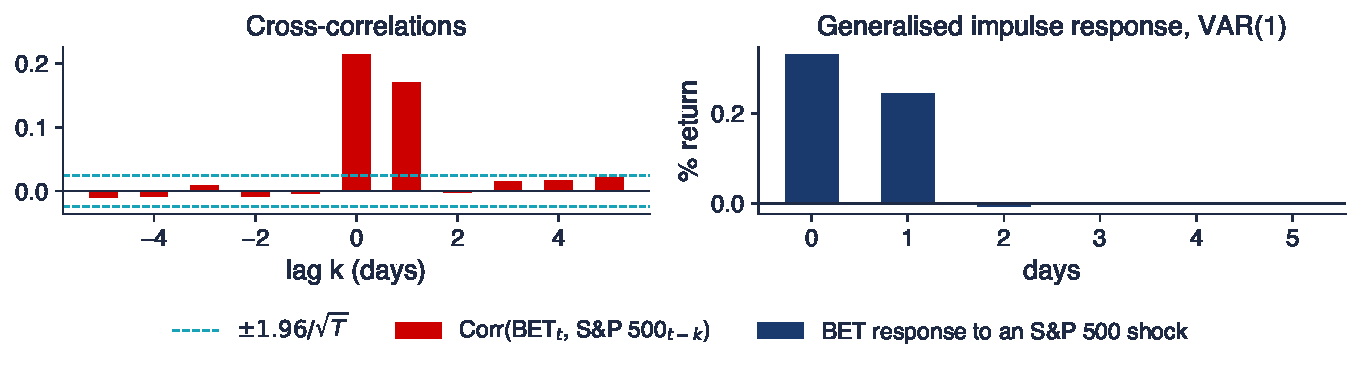
\includegraphics[width=0.96\textwidth,height=0.36\textheight,keepaspectratio]{ch6_sem_b1.pdf}
\end{center}
\vspace{-2mm}
\begin{itemize}
    \item $T = 6\,466$ days; CCF: 0.21 ($k = 0$), 0.170 ($k = 1$), -0.003 ($k = -1$); orders: AIC 9, BIC 1, HQ 1: VAR(1)
    \item S\&P 500 $\to$ BET: $F = 156.2$ (p $<$\,0.001); BET $\to$ S\&P 500: $F = 2.25$ (p 0.133); coefficient of S\&P$_{t-1}$: 0.182 (SE 0.015)
    \item Generalised response of the BET: 0.33\% on the same day, 0.24\% the next day, -0.007\% after two days
    \item Interpretation: Wall Street closes after Bucharest, so news of the American afternoon reaches the BET only the next day: a time-zone effect, not a slow market
\end{itemize}\quantlet{TSA\_ch6\_seminar}{\qlurl{TSA_ch6_seminar}}
\end{frame}

\begin{frame}{B2: the same question with weekly returns [Proposed]}
\itemsize{\footnotesize}
\begin{itemize}
\item \textbf{Question}: does the lead of the S\&P 500 survive when we use Friday-to-Friday weekly returns?
\item \textbf{Inputs}: weekly log returns (\%) of the S\&P 500 and the BET from the Friday closes; model: B1
\item \textbf{Tasks}
\begin{enumerate}
    \item Repeat steps 1--4 of B1 on weekly returns.
    \item Compare the lag-1 cross-correlation and the $F$ statistic with the daily ones.
    \item Interpretation: why is the lead much weaker at the weekly frequency?
\end{enumerate}
\item \textbf{Report}: the same items as in B1 and two sentences
\item Notebook: section B2
\end{itemize}
\end{frame}

\ifsolutions
\begin{frame}{B2: solution [Proposed]}
\itemsize{\scriptsize}
\begin{center}
\includegraphics[width=0.96\textwidth,height=0.34\textheight,keepaspectratio]{ch6_sem_b2.pdf}
\end{center}
\vspace{-2mm}
\begin{itemize}
    \item $T = 1\,379$ weeks; CCF: 0.36 ($k = 0$), 0.063 ($k = 1$); orders: AIC 3, BIC 0, HQ 2: VAR(2)
    \item S\&P 500 $\to$ BET: $F = 4.6$ (p 0.011), against $F = 156.2$ daily; BET $\to$ S\&P 500: p 0.914
    \item Interpretation: the one-day delay now falls inside the same week, so it shows up in the same-week correlation (0.36) instead of the lag; a weak lead remains
\end{itemize}\quantlet{TSA\_ch6\_seminar}{\qlurl{TSA_ch6_seminar}}
\end{frame}
\fi

\begin{frame}{B3: a VAR for the Romanian economy [Solved]}
\itemsize{\footnotesize}
\begin{itemize}
\item \textbf{Question}: how do GDP growth, inflation and the 3-month interest rate interact in Romania?
\item \textbf{Inputs}: $\bY_t = (g_t, \pi_t, i_t)'$, quarterly, 2005Q1--2026Q2
\item \textbf{Tasks}
\begin{enumerate}
    \item Choose $p$ with AIC, BIC and HQ ($p \le 6$) and estimate a VAR(2).
    \item Check stability (largest modulus of the companion eigenvalues) and run the portmanteau test with $h = 8$ and $h = 12$.
    \item Run the six Granger $F$ tests.
    \item Plot the orthogonalised response of ROBOR to an inflation shock (order $g, \pi, i$) and the FEVD of ROBOR.
    \item Interpretation: do the results show that the central bank reacts to inflation?
\end{enumerate}
\item \textbf{Report}: three orders, one modulus, two portmanteau tests, a table of six tests, the chart and one sentence
\item Notebook: section B3
\end{itemize}
\end{frame}

\begin{frame}{B3: solution [Solved]}
\itemsize{\scriptsize}
\begin{center}
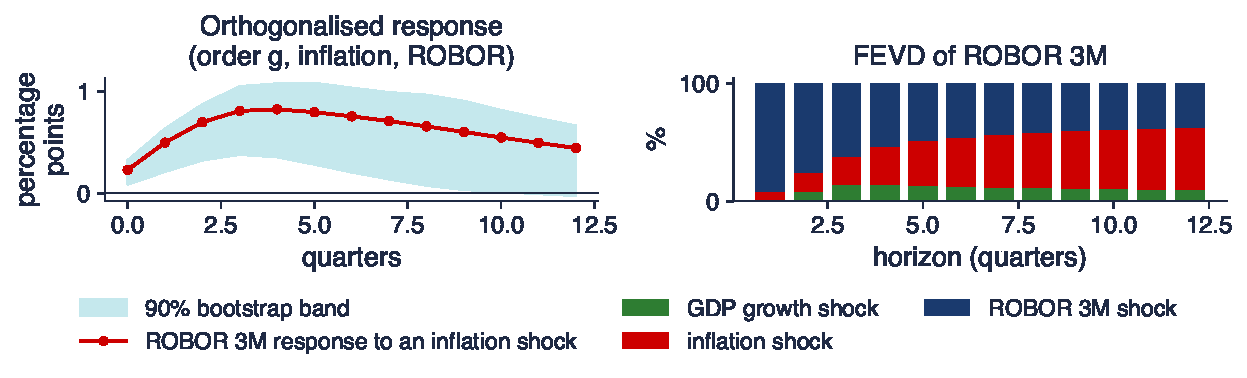
\includegraphics[width=0.96\textwidth,height=0.32\textheight,keepaspectratio]{ch6_sem_b3.pdf}
\end{center}
\vspace{-2mm}
\begin{itemize}
    \item Orders: AIC 5, BIC 1, HQ 2; VAR(2) on 84 quarters; largest modulus 0.869: stable; $Q_8 = 76.7$ (p 0.023), $Q_{12} = 105.3$ (p 0.130)
    \item Granger (p): $g \to i$ 0.001, $\pi \to i$ 0.011, $i \to g$ 0.022, $\pi \to g$ 0.059, $i \to \pi$ 0.417, $g \to \pi$ 0.853
    \item ROBOR after an inflation shock: 0.23 pp on impact, 0.82 pp after 4 quarters; FEVD of ROBOR at 12 quarters: inflation 53\%, own 37\%
    \item Interpretation: they show that ROBOR \textbf{follows} inflation, as a reaction function would imply; ROBOR is a market rate, and the VAR cannot separate the BNR's decisions from market expectations
\end{itemize}\quantlet{TSA\_ch6\_seminar}{\qlurl{TSA_ch6_seminar}}
\end{frame}

\begin{frame}{B4: adding the EUR/RON exchange rate [Proposed]}
\itemsize{\footnotesize}
\begin{itemize}
\item \textbf{Question}: does the depreciation of the leu help to forecast inflation (exchange-rate pass-through)?
\item \textbf{Inputs}: $\bY_t = (g_t, s_t, \pi_t, i_t)'$ with $s_t$ the quarterly EUR/RON change, from 2005Q4; model: B3
\item \textbf{Tasks}
\begin{enumerate}
    \item Choose $p$ with the three criteria ($p \le 4$) and estimate a VAR(2).
    \item Test whether $s$ Granger-causes $\pi$, $i$ and $g$, and whether $i$ and $\pi$ Granger-cause $s$.
    \item Compute the share of EUR/RON shocks in the FEVD of inflation at 1, 4, 8 and 12 quarters.
    \item Interpretation: does the result mean that the exchange rate does not affect Romanian prices?
\end{enumerate}
\item \textbf{Report}: three orders, five $F$ tests, four shares and two sentences
\item Notebook: section B4
\end{itemize}
\end{frame}

\ifsolutions
\begin{frame}{B4: solution [Proposed]}
\itemsize{\scriptsize}
\begin{center}
\includegraphics[width=0.96\textwidth,height=0.32\textheight,keepaspectratio]{ch6_sem_b4.pdf}
\end{center}
\vspace{-2mm}
\begin{itemize}
    \item Orders: AIC 4, BIC 1, HQ 2; VAR(2) on 81 quarters, largest modulus 0.869
    \item $s \to \pi$: $F = 1.41$ (p 0.252); $s \to i$: p 0.281; $s \to g$: p 0.012; $i \to s$: p 0.035; $\pi \to s$: p 0.319
    \item EUR/RON shocks explain 0.3\%, 0.3\%, 0.4\% and 0.5\% of the inflation forecast variance; the response band never excludes zero
    \item Interpretation: no; the leu moved little (a managed float), quarterly averages blur the timing, and 12-month inflation reacts slowly: the test has little power, absence of evidence is not evidence of absence
\end{itemize}\quantlet{TSA\_ch6\_seminar}{\qlurl{TSA_ch6_seminar}}
\end{frame}
\fi


%=============================================================================
\section{Part C: open questions and AI critique}
%=============================================================================

\begin{frame}{C1: the price puzzle [Proposed]}
\itemsize{\footnotesize}
\begin{itemize}
\item \textbf{Question}: why does inflation rise after a ROBOR shock in the VAR of B3, and does it change when the exchange rate or more lags are added?
\item \textbf{Inputs}: the VARs of B3 and B4; ROBOR ordered last; models: B3, B4
\item \textbf{Tasks}
\begin{enumerate}
    \item Plot the response of inflation to a ROBOR shock in the VAR(2) of B3, the VAR(2) of B4 and a VAR(4) with the four variables of B4.
    \item Report the largest and the smallest response and their horizons.
    \item List two pieces of information that the central bank has and the VAR does not.
    \item Interpretation: is a positive response of inflation a proof that higher rates raise prices?
\end{enumerate}
\item \textbf{Report}: the chart, six numbers and a project plan
\item Notebook: section C1
\end{itemize}
\end{frame}

\ifsolutions
\begin{frame}{C1: reference analysis [Proposed]}
\itemsize{\scriptsize}
\begin{center}
\includegraphics[width=0.96\textwidth,height=0.34\textheight,keepaspectratio]{ch6_sem_c1.pdf}
\end{center}
\vspace{-2mm}
\begin{itemize}
    \item Peak response: 0.16 pp after 2 quarters (B3); 0.15 pp after 3 (B4); 0.16 pp after 1 (VAR(4)), then -0.07 pp after 4
    \item The bank sees inflation expectations, energy and food price forecasts, wage data and fiscal plans; when it raises the rate because it expects inflation, the VAR labels the move a ``shock'' followed by inflation
    \item Interpretation: no; it signals a badly identified shock (omitted information), the price puzzle of \refSimsPP
    \item Project: add a commodity price index, the euro-area rate or survey expectations, and compare the responses
\end{itemize}\quantlet{TSA\_ch6\_seminar}{\qlurl{TSA_ch6_seminar}}
\end{frame}
\fi

\begin{frame}{C2: audit an AI answer [Proposed]}
\itemsize{\scriptsize}
\begin{itemize}
    \item A student asked an AI assistant to analyse the VAR of B3. The answer:
    \item \aiprompt{(a) AIC chooses p = 5, so the true lag order of the economy is 5.}
    \item \aiprompt{(b) The largest eigenvalue modulus of A1 is 1.37, so the VAR(2) is explosive.}
    \item \aiprompt{(c) The portmanteau test at 8 lags has p = 0.023, so the residuals are white noise.}
    \item \aiprompt{(d) GDP growth Granger-causes ROBOR, so faster growth causes the BNR to raise rates.}
    \item \aiprompt{(e) Cholesky impulse responses do not depend on the order of the variables.}
    \item \aiprompt{(f) In each row of the FEVD the shares add up to 100\%.}
    \item Tasks
    \begin{itemize}
        \item 1. For each statement, say whether it is correct; if not, give the correct statement and, where possible, the correct number from the notebook (section C2).
        \item 2. Report: a list of six verdicts with one line of justification each.
    \end{itemize}
\end{itemize}
\end{frame}

\ifsolutions
\begin{frame}{C2: solution [Proposed]}
\itemsize{\scriptsize}
\begin{itemize}
    \item (a) Wrong: criteria choose a model for a sample; BIC chooses 1, HQ 2; there is no ``true'' order to discover
    \item (b) Wrong: the stability of a VAR(2) is decided by the companion matrix; its largest modulus is 0.87 $< 1$: stable
    \item (c) Wrong: p = 0.023 $< 0.05$ rejects white noise at 8 lags (at 12 lags it is not rejected)
    \item (d) Wrong: Granger causality is predictability; ROBOR is a market rate and both may react to a third factor
    \item (e) Wrong: the order decides which variable reacts on impact (A3, B3)
    \item (f) Correct
\end{itemize}\quantlet{TSA\_ch6\_seminar}{\qlurl{TSA_ch6_seminar}}
\end{frame}
\fi


%=============================================================================
\section{Wrap-up}
%=============================================================================

\begin{frame}{Key takeaways}
\itemsize{\small}
\begin{itemize}
    \item Stability: eigenvalues of $\bA$ (or of the companion matrix) inside the unit circle; then forecasts converge to $\boldsymbol{\mu}$
    \item Granger $F$ test: compare the equation with and without the lags of the candidate variable
    \item Cholesky responses depend on the ordering; the generalised responses do not
    \item S\&P 500 leads the BET by one day because of the time zones; ROBOR follows Romanian inflation
    \item An AI answer is a draft: check the direction of each claim and which matrix decides stability
\end{itemize}
\end{frame}

\begin{frame}{After the seminar}
\itemsize{\small}
\begin{itemize}
    \item Lecture 6 develops each topic of today: vector processes, the companion form, lag selection, diagnostics, Granger causality and its pitfalls, impulse responses, FEVD, spillovers, forecasting, structural VARs
    \item Try the [Proposed] tasks in the notebook
    \item C1 can grow into a team project: monetary policy shocks in Romania with an extended VAR
    \item Reading: \refHP, Ch.~7; \refFPP, Sec.~12.3; \refSW
    \item \textbf{The seminar is for practice and is not graded; the solutions of [Proposed] tasks are discussed in class}
\end{itemize}
\end{frame}


%=============================================================================
\section{References}
%=============================================================================

\begin{frame}{References}
\itemsize{\tiny}
\begin{itemize}
    \item Granger, C. W. J. (1969). Investigating causal relations by econometric models and cross-spectral methods. \textit{Econometrica}, 37(3), 424--438. \href{https://doi.org/10.2307/1912791}{doi:10.2307/1912791}
    \item Huang, C., \& Petukhina, A. (2022). \textit{Applied Time Series Analysis and Forecasting with Python}. Springer. \href{https://doi.org/10.1007/978-3-031-13584-2}{doi:10.1007/978-3-031-13584-2}
    \item Hyndman, R. J., \& Athanasopoulos, G. (2021). \textit{Forecasting: Principles and Practice} (3rd ed.), Section 12.3, Vector autoregressions. OTexts. \href{https://otexts.com/fpp3/VAR.html}{otexts.com/fpp3/VAR.html}
    \item Lütkepohl, H. (2005). \textit{New Introduction to Multiple Time Series Analysis}. Springer. \href{https://doi.org/10.1007/978-3-540-27752-1}{doi:10.1007/978-3-540-27752-1}
    \item Pesaran, M. H., \& Shin, Y. (1998). Generalized impulse response analysis in linear multivariate models. \textit{Economics Letters}, 58(1), 17--29. \href{https://doi.org/10.1016/S0165-1765(97)00214-0}{doi:10.1016/S0165-1765(97)00214-0}
    \item Sims, C. A. (1980). Macroeconomics and reality. \textit{Econometrica}, 48(1), 1--48. \href{https://doi.org/10.2307/1912017}{doi:10.2307/1912017}
    \item Sims, C. A. (1992). Interpreting the macroeconomic time series facts: The effects of monetary policy. \textit{European Economic Review}, 36(5), 975--1000. \href{https://doi.org/10.1016/0014-2921(92)90041-T}{doi:10.1016/0014-2921(92)90041-T}
    \item Stock, J. H., \& Watson, M. W. (2001). Vector autoregressions. \textit{Journal of Economic Perspectives}, 15(4), 101--115. \href{https://doi.org/10.1257/jep.15.4.101}{doi:10.1257/jep.15.4.101}
\end{itemize}
\end{frame}

\end{document}
